\chapter{Methods}
This chapter introduces the methodology and system architecture followed by the experimental designs for the quantitative analysis.
The system architecture describes the GNU Radio flow-graph description, software and hardware used in this project. The experiments are presented in chronological order. In the first experiment, the performance of the system is measured with respect to broader parameters like sampling rate and data payload size. The second experiment was designed evaluation of the impact of these parameters on the the different subsections of the data path. In experiment 3, the project looks at the impact of the USB transfer size on the overall delay.

\section{Methodology}
This project uses quantitative experimental design method.
The characterization of timing delays needs to have quantitative measurements as they would help compare it to the specified standards and define the limitations concretely.
This project concentrates on designing experiments for understanding the causal effect of system parameters on the measurements.\\

A method was needed for measuring the time duration of the individual process as this project aims for timing characterization of signal processing chains.
The LimeSDR doesn't have a real time clock on board, so in order to measure time on the LimeSDR, it was needed to synchronize different clock domains across a variable latency link.
This process is complex and not feasible given the time constraint, so this project avoids doing any time measurement on the LimeSDR.
Taking hints from the literature review, this project opts to timestamp the \ac{sdr} software processes on the host computer.
This method is reliable and doesn't affect the measurements significantly.\\

Most of the previous studies used ping as the measurement tool.
In this case, there are two host computer connected through two \ac{sdr} platforms.
As the host computers will not be identical they will impact the collected measurement differently.
It would also not be possible to evaluate the impact of the host computer processing resources in this case.
Another problem with this method is the use of common frequency bands, communication among other devices can make the setup unreliable.
As this project concentrates on the performance of the LimeSDR platform without considering the channel conditions, the impact of communication through the air medium can be safely ignored.
Finally, measurement across two different platforms makes it difficult to correlate the measurements on the two computer as the clocks are not synchronized.
Considering these factors, this project picked the loopback method.
In this method, the TX and RX chains on the LimeSDR are shorted before the \ac{LNA} of the LMS7002M chip shown in Figure \ref{lms7002m}.
This method uses the radio frontend of the LimeSDR which helps evaluate the impact of radio-frontend configuration on the performance.




\section{Experimental Setup}
The physical experimental setup is shown in Figure \ref{Real_Setup} to provide the broader picture of the setup.
The host computer is running the GNU Radio communication system which interacts with the LimeSDR platform through \ac{USB} 3.0 connection.
The LimeSDR has been configured to run in the loop back configuration.\\

\begin{figure}[h!]
\centering
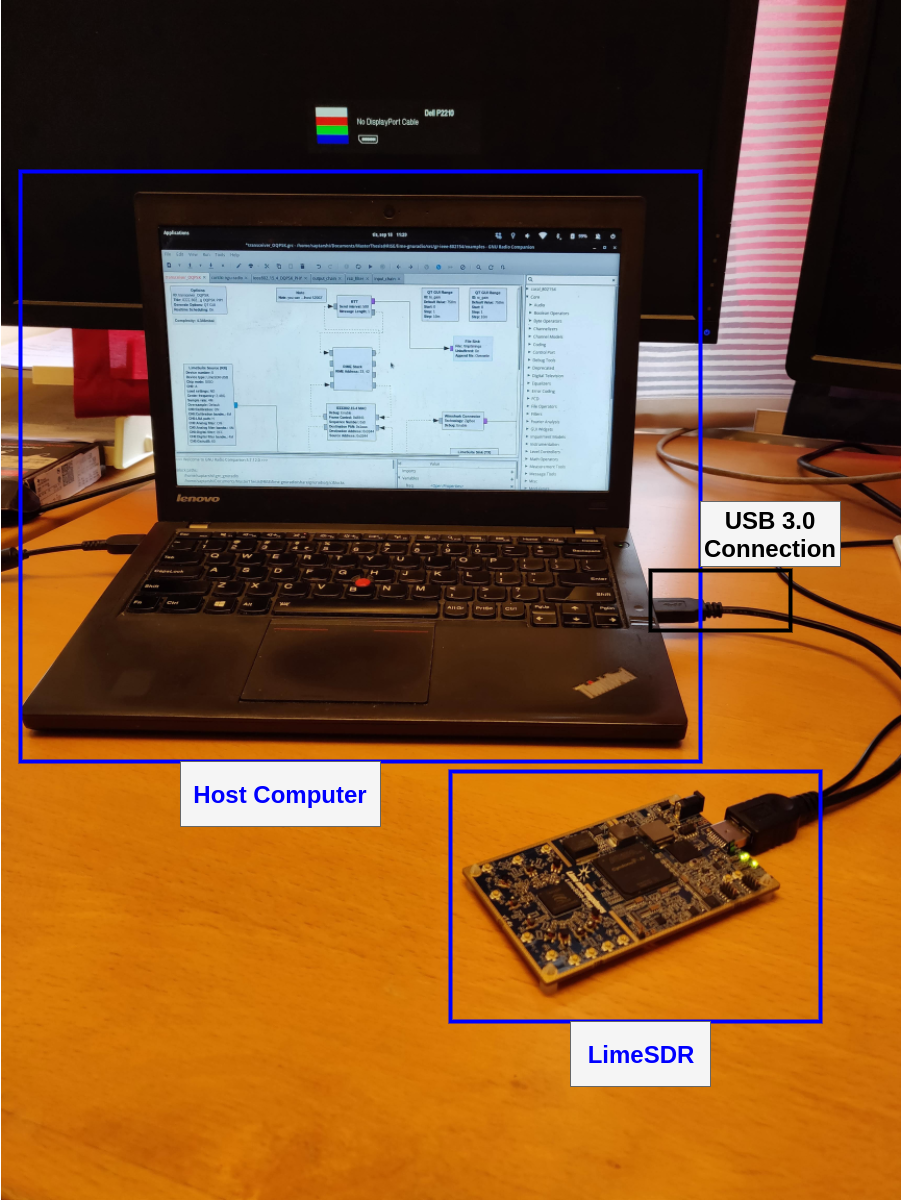
\includegraphics[scale=0.2]{Thesis/Figure/MeasurementSetup.png}
\caption{Measurement Setup}
\label{Real_Setup}
\end{figure}

\begin{figure}[h!]
\centering
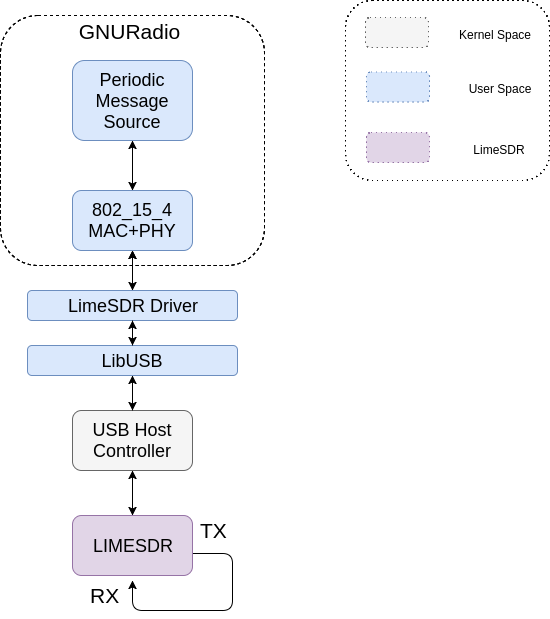
\includegraphics[scale=0.6]{Thesis/Figure/Setup_Description.png}
\caption{Experimental Setup Flow Diagram}
\label{Experimental_Setup_Flow_Digram}
\end{figure}


The software flow diagram for the experimental setup is shown in Figure \ref{Experimental_Setup_Flow_Digram}.
This diagram in conjunction to the dataflow diagram (Figure \ref{Dataflow}) gives the complete picture of the experimental setup.
In figure \ref{Experimental_Setup_Flow_Digram}, the GNU Radio runs the communication system which is primarily based on the WIME project implementation of 802.15.4 protocol.
A message source block, described in \ref{Periodic Message Source}, is added which helps in generate controlled excitation signal for evaluating the experimental setup.
It generates the payload for the \ac{mac} layer of the Wime 802.15.4 MAC, which adds the MAC header and the \ac{CRC} for the MAC packet.
The Wime 802.15.4 PHY adds the preamble and the length fields for the physical layer packet.
This physical layer packet is modulated through the O-QPSK modulation.
The GNU Radio processes these samples in chunks, the chunk size defined by the block's scheduler.
The samples generated by this GNU Radio process is passed to the LimeSDR driver which does the process described in \ref{TX Data Path}.
It generates the FPGA packets in batches, with the batchsize defined at initialization.
The formatted packets are forwarded to libusb which generates the USB transaction and finally the host controller transfers the data to the LimeSDR.
Each USB transaction has a token defining the direction of the transfer, followed by the bursts of USB data packets.
The size of the USB data packets is defined by the USB descriptor of the LimeSDR Cypress EZ FX3 during device registration.

\begin{figure}[h!]
\centering
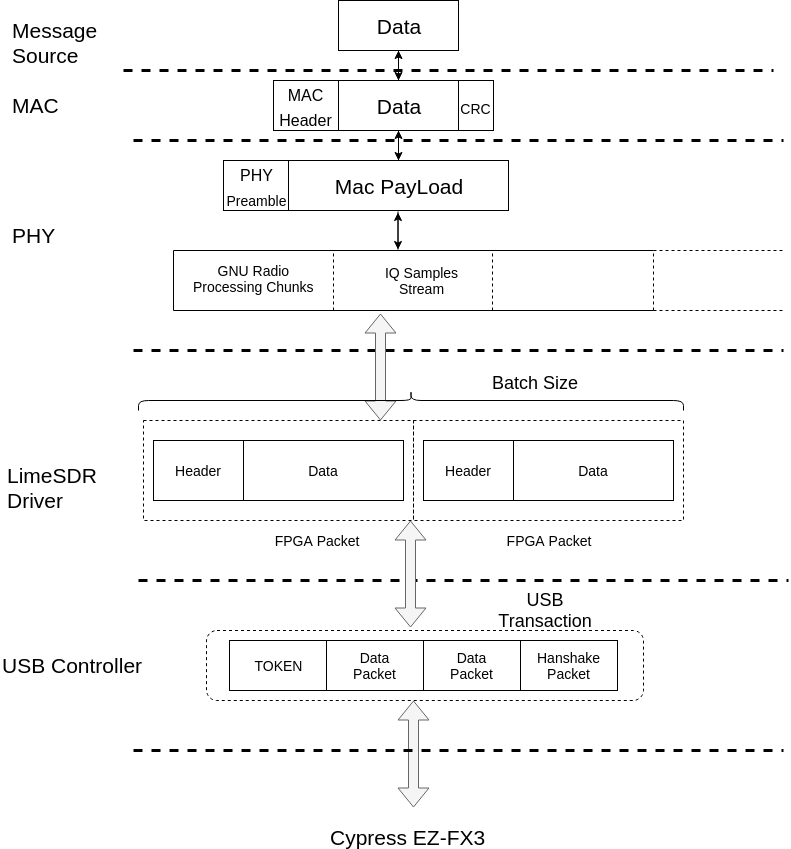
\includegraphics[width=0.8\textwidth]{Thesis/Figure/Dataflow.png}
\caption{Dataflow Diagram}
\label{Dataflow}
\end{figure}


\subsection{Adaptations}
The Wime project implementation needed to be modified to use LimeSDR instead of USRP as the \ac{sdr} platform.
Furthermore, the entire experimental setup needed some alterations to facilitate the experiemental process.These adaptations can be grouped as:

\begin{enumerate}
\item{GNU Radio Source and Sink blocks}
\item{802.15.4 \ac{PHY} layer}
\item{Periodic Message Source}
\end{enumerate}

\paragraph{GNU Radio Source and Sink Blocks}
The USRP source and sink blocks are replaced by the gr-limesdr source and sink blocks for using the LimeSDR platform.
Another alternative used in this project is the gr-osmosdr sink and source blocks which used soapysdr to access the Lime API. The former was chosen as it directly interacts with the LimeAPI without using the adaptation layer presented by the soapysdr project. This gives much better control of the board control parameters and also saves multiple \textit{memcpy} operations used by the soapysdr adaptation layer.\\

In both these blocks, the loopback configuration is defined at initialization by setting the loopback register on the NIOS processor.
This turns on the switch at the end of the \ac{LNA} which creates a data flow from the TX path to the RX data path on the LMS7002M.\\


LimeSDR driver sends USB packets in bursts whose size is determined by the FPGA data packet size and the batchsize of FPGA data packet defined for the stream.
In case, the GNU Radio packet data size is less than the size of a burst, the Streamer function of the driver waits for more data from the GNU Radio.
It pads zeros after the end of the original data and sends the burst data after a set timeout.\\

\begin{figure}[h!]
\centering
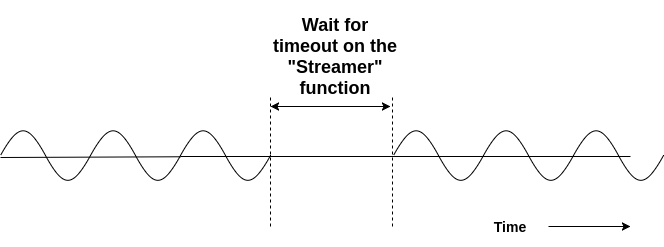
\includegraphics[scale=0.6]{Thesis/Figure/SilentProblem.png}
\caption{Radio Silent Problem}
\label{Radio_Silent}
\end{figure}

This implementation works well for continuous stream based protocols, but for packet based protocols like the IEEE 802.15.4 this leads to radio silence problem, as illustrated in Figure \ref{Radio_Silent}.
In this figure, an example LimeSDR transmission over the air is shown.
If the data contained in one packet doesn't satisfy the size requirement imposed by the LimeSDR driver, the radio becomes silent(shown as the gap in the figure) and the transmission breaks down.
The receiver assumes that the radio signal for a packet is a single continuous stream, so if the radio signal is interrupted then it can not receive the packet properly.\\

This project adds a GNU Radio stream tag called "End of Packet" to the end of sample stream from the 802.15.4 PHY block for solving this problem.
In the gr-limesdr block, the tag instructs the Streamer function of the driver to immediately send the data to the LimeSDR by appending zeros at the end of the packet data.

\paragraph{802.15.4 \ac{PHY} layer}

The WIME project \ac{PHY} layer has been designed to only work with 4 MHz as the sampling rate, in this project, the \ac{PHY} layer has been modified to accommodate different sampling rates as it helps in understanding the impact of sampling rate on the performance.\\

On the TX flowgraph of the GNU Radio 802.15.4, \ac{PHY} a sine wave generator is added which takes the desired frequency as input.
The "Repeat" block interpolates a single chip by repeating it $set frequency/1 MHz$ times as the modulator generates a signal of bandwidth 1 MHz.
On the RX flowgraph, the clock recovery module decimates by $set frequency/2 MHz$ as the received signal should have a bandwidth of 2 MHz.

\paragraph{Periodic Message Source} \label{Periodic Message Source}
This project needed a controllable excitation source for evaluating the experimental setup.
A periodic message source block was implemented in the GNU Radio, it takes in the message length and time period as parameters.
Figure \ref{message_source} shows the working of the message source with respect to time.
The time period controls the time duration between two subsequent message generation.
The data length controls the data payload size of the 802.15.4 \ac{mac} packet.
It indirectly controls the transmission time,$\Delta T_{tx}$, of the the message.
The larger the message payload, the more time it will take to transmit through the setup. 
\\

\begin{figure}[h!]
\centering
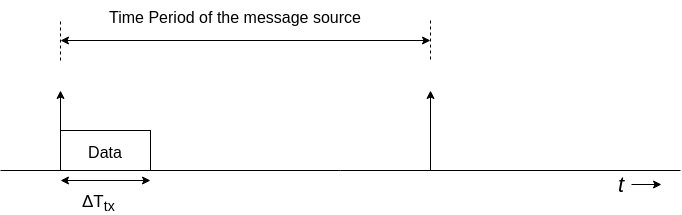
\includegraphics[width=\textwidth]{Figure/Message_Source.png}
\caption{Periodic Message Source}
\label{message_source}
\end{figure}

\subsection{Hardware and Software Used}

\section{Experiment 1: Impact of network parameters on latency}

The first experiment is designed to evaluate the impact of network parameters on the the latency.
Before going into the details of the experiment, this report needs to explain this project's definition of latency.

\subsection{Latency}
In general, the latency is defined as the time it takes a packet to reach the receiver from the transmitter.
In this project, the transmission time is defined the time the packet enters the 802.15.4 \ac{mac}.
And, the reception time is defined as the time the SFD is detected in the received packet by the 802.15.4 PHY packet detector.\\

This latency definition is asymmetric, and it ignores the processing time of received packers in the \ac{mac} layer. So all the reported values are lower than the those for MAC layer latency.
This is done to eliminate the impact of throughput on the latency measurements, as the study concentrates mainly on the time delay analysis.\\

The periodic message source notes down the global system time as $T_1$ when it publishes a message to its output port.
This value is written to a file when the message source receives the payload from the MAC, this ensures that time for data packets successfully decoded by the \ac{mac} is only noted.
The packet detector in the RX flow-graph detects the SFD and notes down the time as $T_2$.
When the entire packet is successfully decoded by the packet detector, it writes this time to another file.
The decoding of the entire packet makes sure that the program only writes the time for a physical layer packet not whenever it detects the preamble sequence.\\

Since the time noted should be compared with those from usbmon, $clock\_{gettime}$ was selected as the preferred method. 
The difference $T_2 - T_1$ will give the latency as per this project's definition.
As two different processes are measuring the time-stamps, the correct $T_1$ and $T_2$ needs to be grouped together for the latency measurement. 
The following algorithm is used for this purpose.

\begin{algorithm}[!h]
\caption{Time Data Correlation}
\begin{algorithmic}
\State {$T \gets $ Time Period of Message Source }
\State {$l \gets $ min(length of time arrays)}
\State $i \gets 0$
\For {$i < l $}
\If{($ t1[i]> t2[i] $)} \\
\hspace{1.35cm} delete $t1[i]$
\ElsIf{$(t2[i]-t1[i]) > T $}
delete t2[i]
\Else{ $i \gets i+1$ \\ \hspace{1.35cm} $l \gets $ min(length of time arrays) }
\EndIf
\EndFor
\end{algorithmic}
\end{algorithm}
It is assumed that the time period of the message source is greater than the latency.\\

\subsection{Experiment Design}
The impact of amount of data sent to the LimeSDR and the impact of higher sampling rate on the latency needs to be evaluated.
\begin{itemize}
    \item {\textbf{Objective} These parameters would help quantitatively analyze if this system design can also be applied for running higher bandwidth protocols like IEEE 802.11ac.
Another goal of performing this experiment, is to validate the timestamp method for the latency analysis.
In ideal case, the latency shouldn't be dependent on the amount of data or the sampling rate.}
\item{\textbf{Input Parameters} The experiment has two input parameters:
\begin{enumerate}
    \item {The length of the messages generated by the periodic message source block.
    Since the PHY payload for 802.15.4 should be less than 128 bytes, the message source data length plus MAC header should be less than that.
    The maximum message source data length comes to be 112 bytes with MAC header of 15 bytes.
    The project decided to spread the message source length across the entire available range from one to 112.
    We choose four different message sizes: 1 byte ,37 bytes,74 bytes and 112 bytes.}
    \item {The sampling rate, which defines the interpolation and decimation ratio in the 802.15.4 physical layer.
    It also configures the FPGA sampling clock.
    More samples needs to be processed for higher sampling rates.
    The default sampling rate for 802.15.4 is 4 MHz, this project also adds 8 MHz and 16 MHz as sampling rate to get an idea on the impact of a protocol's bandwidth requirements on performance.
    }
\end{enumerate}
}
\item{\textbf{Output Metric} The latency which is defined by the previous subsection as $T_2 - T_1$}
\item{\textbf{Design of the experiment} Firstly, the time period of message source was set to 500ms to ensure that the individual latency measurement are independent of each other.
The LimeSDR FPGA data packet batchsize is set to one.
A python script was created to automate the process, which runs the process for 100 seconds.
The message source generates 199 packets during this duration which gives us 199 latency measurements.
}
\end{itemize}

\section{Experiment 2: Analysis of component delays}
Granular timestamps are necessary for quantitatively analyzing the results from Experiment 1.
These also helps the project figuring out the bottlenecks in this system architecture and to comprehensively fill up the knowledge gap discovered by the literature review.
This project defines seven different time delays for this purpose.
\begin{enumerate}
    \item {\textbf{GNU Radio TX Processing Delay} This provides the delays incurred to generate the sample stream of the modulated packet.}
    \item{\textbf{LimeSDR TX Driver Delay} The time it takes the driver to pack the data into batches of FPGA data packet can be an important metric to show if the driver needs a closer look for optimization. } 
    \item{\textbf{User Space to Kernel Space Delay} This delays gives an idea how the Linux process scheduler impacts the performance.
    }
    \item{\textbf{LimeSDR loopback Delay} The time taken by the bus transfer, the buffering in the LimeSDR FIFOs  and the hardware delays provides an insight how the transfer of  data from Host Computer to the LimeSDR and vice-versa impacts the performance.
    In this case, the project assumes the hardware processing delays are negligible and most of the time is contributed by the bus transfers and buffering delays.
    }
    \item{\textbf{Kernel Space to User Space Delay} It focuses on the impact of linux scheduling.
    }
    \item{\textbf{LimeSDR RX Driver Delay} It provides the time needed to unpack the FPGA data packets and pass them to the GNU Radio flow-graph.
    It also includes the buffering time in case the GNU Radio RX flow-graph is unable to process the samples in real-time.
    By real-time, this project means the data cannot be processed at the rate they are being generated.}
    \item{\textbf{GNU Radio RX Processing Delay} It provides the delays introduced by the RX flow-graph in GNU Radio.}
    
\end{enumerate}

\subsection{Component Time Delays Measurement}
 With the need for fine-tuning the delay measurement highlighted, this report concentrates on providing the implementation details of this measurement setup.\\
 
 \begin{figure}[h!]
\centering
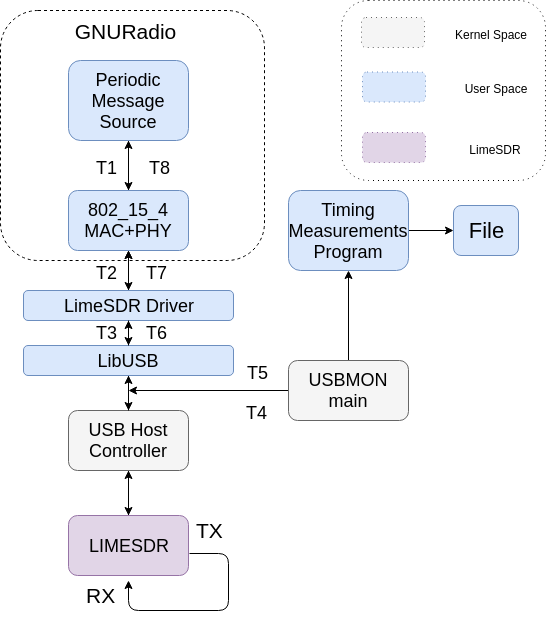
\includegraphics[width=0.8\textwidth]{Figure/Setup2.png}
\caption{Component Time Delay Measurement Setup}
\label{component_setup}
\end{figure}

The measurement setup for this experiment has been shown in Figure \ref{component_setup}.
This setup is more or less similar to our initial setup, with the timestamp data points enumerated as per the delays mentioned previously.
The timestamps $T_1$ and $T_2$ described in Experiment 1, will henceforth be referred to as $T_1$ and $T_8$ respectively for the rest of the report.
The project concentrated on finding the last execution statement applied to the data in each component,shown in Figure \ref{component_setup}, using static code analysis.
This method is only valid for the user space components as the source code for them is easily accessible.
The method for measurement of the timestamp from the USB Host Controller in kernel space is complicated and will be covered in the next subsection.\\

 \begin{figure}[h!]
\centering
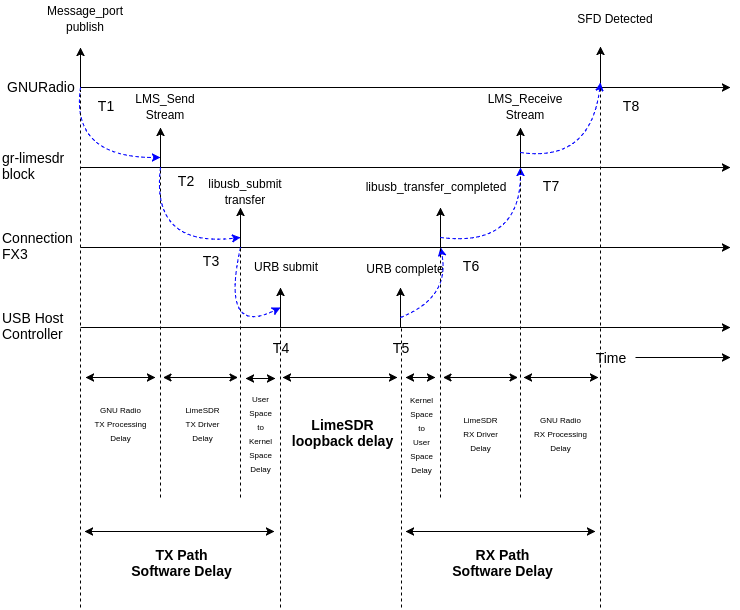
\includegraphics[width=\textwidth]{Thesis/Figure/Timepoints.png}
\caption{Overview of the timestamps.}
\label{time_points}
\end{figure}

The timestamps, their corresponding execution calls , and how they relate to the delays defined previously have been shown in Figure \ref{time_points}. 
Starting with the TX path, we have the time the message enters the \ac{mac} layer of the 802.15.4 as $T_1$ from the previous experiment, LMS\_SendStream on the gr-limesdr block hands over the data to the LimeSDR driver.
So a timestamp is taken just before the LMS\_SendStream call which is referred as $T_2$.
The difference $T_2 - T_1$ gives the GNU Radio TX Processing Delay.
The LimeSDR driver uses the Connection FX3 module for interacting with the libusb library.
The time instant the data is handed over to the libusb library using the libusb\_submit\_transfer is noted down as $T_3$.
$T_3 - T_2$ gives us the time taken by the LimeSDR driver on the TX Path.
When the data is sent to the USB Host Controller using URB\_submit from the kernel \ac{USB} driver, we measure the time of the first transfer of a 802.15.4 TX data packet as $T_4$.
The difference gives us $T_4 - T_3$ the time it takes for the data to be sent to the USB host controller referred as User Space to Kernel Space Delay.\\

Coming to the RX data path, the time for the first transfer of a 802.15.4 RX packet data from the USB Host Controller to the kernel \ac{USB} driver is noted as $T_5$.
The LimeSDR loopback delay can be measured from the $T_5 - T_4$.
When the Connection FX3 module in the LimeSDR driver receives a USB transfer, the timestamp $T_6$ is taken.
The kernel space to user space delay is taken as $T_6 - T_5$.
$T_7$ is measured when the gr-limesdr blocks receives the data using LMS\_ReceiveStream.
$T_7 - T_6$ gives us the delay introduced by the LimeSDR driver on the RX data path.
Finally we have $T_8$ from our previous experimentation, which provides $T_8 - T_7$ as the GNU Radio RX processing time.\\


\subsection{Measuring $T_4$ and $T_5$}
In order to ensure that the LimeSDR loopback delay is as accurate as possible to the delay contributed by the buffering and hardware delays, this project picks USB Host Controller as the source for measurement of $T_4$ and $T_5$.
The measurement method is complicated by this choice.
Firstly, modifying the USB Host Controller code is complicated.
Secondly, the measurement value of $T_4$ and $T_5$ should be for only 802.15.4 packets and not all TX and RX data, as it would provide the bounds for our data correlation.\\

The project uses the USBmon kernel utility to monitor the $urb\_submit$ and $urb\_request $ calls to and from the \ac{USB} Host Controller.
Each URB has an associated timestamp which is generated by the kernel \ac{USB} driver and the \ac{USB} Host Controller for submit and request respectively.
The project uses the binary interface of the USBmon main utility as the text interface provides only 64 bytes of URB data which is not suitable for our use case.
Once the events have been received from the USBmon event queue, it necessary to find the relevant USB transfers in these events.
This project adopts an offline processing approach, where as separate program "Timing Measurement Program" (shown in Figure \ref{component_setup}) collects all the events, filters out the unnecessary event data and writes the remaining to files.
This approach is chosen as the online data processing approach adds processing overhead which will impact the component delays.
Furthermore, this approach provides us the USB Transfer data which can be used for further processing if necessary.

\paragraph{Timing Measurement Program}
The timing measurement program can be explained using flowchart as shown in Figure \ref{program}
This program uses ioctl to access the /dev/usbmonX character device which allows it to access the USBmon kernel utility event queue.
The events are filtered to find transfers with data endpoints, 0x01 and 0x81 (shown in Table \ref{Lime-USB_ep}), which are written to TX datafile and RX datafile respectively.
 \begin{figure}[h!]
\centering
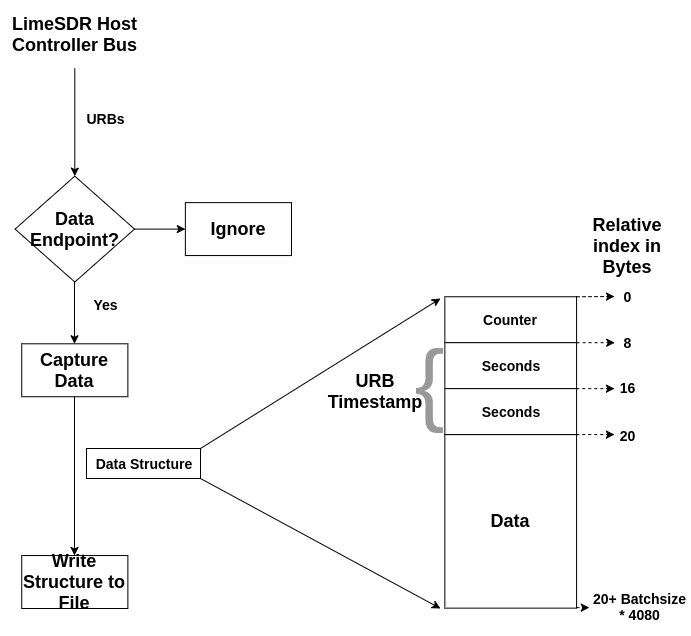
\includegraphics[scale=0.5]{Thesis/Figure/Program_DataStructure.png}
\caption{Timing Measurement Program flow chart}
\label{program}
\end{figure}
The data is buffered in a memory before writing in file as it results in less frequent calls to the file write operation.
A data structure is defined for helping the analysis program to parse through the written data files which is shown in Figure \ref{program}.
The structure includes a eight bytes counter, which shows the sequence number of the structure, it is used primarily for debugging.
The URB timestamp is added to the structure, it is subdivided into eight bytes for the seconds value of the timer and four bytes for fractional seconds which provides the timer value in microseconds.
One thing to note here is that the USBmon measures time using $clock\_gettime$ provided by the the linux time library.
In order to relate all the timestamps together, all the other timestamps are measured using the same method.
The timing measurement program strips away the LimeSDR FPGA data packet header and clubs all the data in one \ac{USB} transfer in the data field of this structure.
The default FPGA packet contains 4080 bytes of data, so the amount of data written will be $Batchsize \times 4080$, which is shown in Figure \ref{program}

\paragraph{USB Data Analysis}
\begin{figure}[h!]
\centering
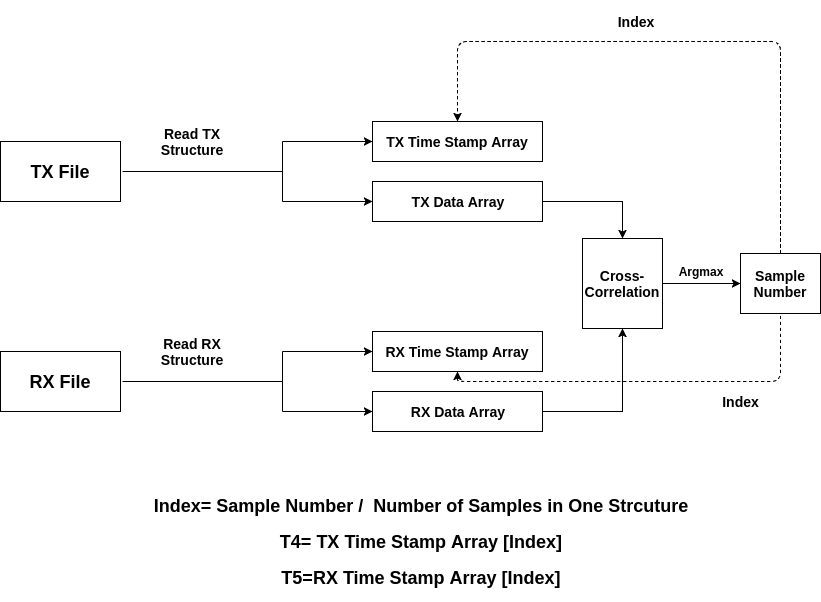
\includegraphics[width=0.8\textwidth]{Thesis/Figure/data_corr.png}
\caption{USB Data Analysis Program Structure}
\label{usb_analysis}
\end{figure}

The data structures written to the TX datafile and RX datafile needs to be analyzed to find the timestamps $T_4$ and $T_5$ respectively.
Since this project uses analog loopback, the TX sample value changes as it is converted to analog and again  sampled to digital RX samples.
For this reason, the sample values in the TX and RX USB packets can not be compared to find when the same sample is returned.
Hence, this project uses cross-correlation to match the TX and RX USB transfers and find the time shift of the RX samples from the TX samples.\\

The structure of the program written for this purpose is shown in Figure \ref{usb_analysis}.
The program starts off by reading the TX data file, it parses the data structure to find the data samples.
It writes the data samples to the TX Data Array when the amplitude of some samples is greater than 0.5.
This value is chosen as a threshold to check for relevant data after experimental observation.
The URB time-stamp in the structure is written to the TX timestamp array.
The program then writes the subsequent structures to a data array and timestamp array until the URB timestamp exceeds the first timestamp by 500 $\mu s$.
Again, this value is chosen by experimental observation.
The first URB timestamp in the the TX timestamp array is chosen as $T_4$ as it is the timestamp for the first relevant TX \ac{USB} transfer.\\

The RX data file is parsed for a \ac{USB} transfer which was received just after $T_4$.
The data of the structures containing this transfer and subsequent transfers are written to the RX data array and the URB time stamps are written to the RX timestamp array.
Once the data has been structured in this array, they are converted to complex data samples using the method used by the LimeSDR RX Driver.
The complex data samples are then cross-correlated with the TX data array, and the sample index for the maximum cross-correlation value is found.
When the first sample of the TX sample is perfectly aligned with the first RX sample it will be given the maximum cross-correlation value.
The cross-correlation maximum sample index gives the sample index of the first relevant RX sample as the TX samples do not have any initial shift because of the previous structuring.\\

Now, the URB timestamp for that sample is found by the following equations
\begin{equation}
    \centering
    RXTime_{index}=\frac{argmax(TX_{data} \star RX_{data})}{N \times Batchsize}
    \label{index}
\end{equation}

\begin{equation}
    \centering
    T_5 = RX Time Array[\floor*{RXTime_{index}}]
    \label{t5}
\end{equation}

where $\star$ is cross-correlation operator, N is the number of samples in one LimeSDR FPGA packet (default value is 1020 samples) and $\floor*{.}$ is the mathematical floor function.\\

Equation \ref{index} provides the index for the RX Time Array which is used to generate $T_5$, the URB timestamp for the first relevant RX USB transfer.

\subsection{Data Correlation} \label{data_corr}

$T_2$,$T_3$,$T_6$ and $T_7$ are measured for all the calls to their corresponding execution statements.
As the LimeSDR is continuously streaming data, the timestamps for the relevant execution calls needs to found out.
This problem has been highlighted for the RX data path using Figure \ref{corr_problem}.\\
\begin{figure}[h!]
\centering
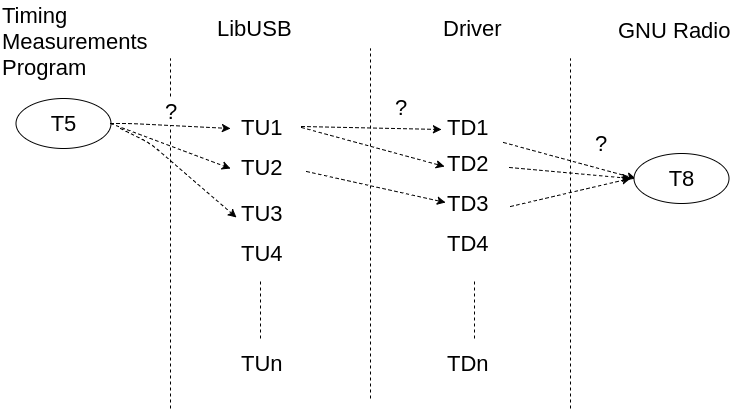
\includegraphics[width=0.8\textwidth]{Thesis/Figure/events.png}
\caption{TimeStamp Correlation problem}
\label{corr_problem}
\end{figure}

From the timing measurements program we derive $T_5$, which is the time for the first relevant RX USB transfer when a message is loop-backed.
We also know $T_8$ from the GNU Radio.
But the continuous stream of RX samples from the LimeSDR results in multiple calls to the libusb and driver timestamps measurements shown in Figure \ref{corr_problem} as $TD_x$ and $TU_x$.
So measure the corresponding delays we need to figure out out which $TD_x$ and $TU_x$ should be picked given $T_5$ and $T_8$. \\


This project avoids doing this check at runtime at each component as it is difficult to find the relevant data in a sample stream and also it adds unnecessary overhead which will impact the measured delays.
We use the knowledge that the timestamps should be such that $T_8>T_7>T_6>T_5$, to find all possible values of $T_6$ and $T_7$ which satisfy this condition.
We defined $T_5$ as the time the first RX USB packet is detected, so we take the first value of $T_6$ and $T_7$ which satisfies the condition. This process has been explained using algorithm \ref{data}.
The algorithm assumes that the $T_5$ value is correct, it then searches for $T_6$ that is greater than $T_5$ because of the condition defined before.
Once $T_6$ has been determined, it looks for $T_7$ that is just greater than $T_6$.
Similarly $T_8$ greater than $T_7$ is found.
One limitation with this measurement is that we cannot correlate all the timestamps.
This process is similar for the TX data path.

\begin{algorithm}[!h]
\caption{Data Correlation}
\begin{algorithmic}
\State {$T \gets $ Time Period of Message Source }
\State {$l \gets $ min(length of time arrays)}
\State $i \gets 0$
\State $j \gets 0$
\State $k \gets 0$
\State $m \gets 0$
\State $flag \gets 0$
\For {$i < l $}
\hspace{1.35cm}\While {($T_5[i] >= T_6[j])$}\\
\hspace{1.70cm}$j \gets j+1$
\EndWhile
\hspace{1.35cm}\While {($T_6[j] >= T_7[k])$}\\
\hspace{1.7cm}$k \gets k+1$
\EndWhile
\hspace{1.35cm}\While {($T_8[m] >= T_7[k])$}\\
\hspace{1.7cm}$m \gets m+1$
\EndWhile
\hspace{1.35cm}\State $\Delta_{GNU Radio}[i] \gets T_8[m]-T_7[k]$
\hspace{1.35cm}\State $\Delta_{Driver}[i] \gets T_7[k]-T_6[j]$
\hspace{1.35cm}\State $\Delta_{Kernel}[i] \gets T_6[m]-T_5[i]$
\EndFor
\end{algorithmic}
\label{data}
\end{algorithm}

\subsection{Experiment Design}
This experiment aims to find out the delays in different software and hardware components in the system architecture shown in Figure \ref{component_setup}.
\begin{itemize}
    \item {\textbf{Objective} This experiment will provide comprehensive understanding of the system and how different input parameters and host computer configuration affect the system performance.
Furthermore, this understanding will help future delay mitigation work.}
\item{\textbf{Input Paramters} The experiment has been designed to investigate the impact of message sizes.
As evident from the results of experiment 1, sampling rate of 4 MHz results in the least variation of latency with message sizes.
So it is chosen as the sampling rate for this experiment.
We chose three message sizes for this experimenent: 1 byte, 56 bytes and 112 bytes.}
\item{\textbf{Output Metrics} The components delays are the output metrics for this experiment.
The component delay and their relation with timestamps defined previously is summarized below (shown graphically in Figure \ref{time_points}).
\begin{itemize}
    \item GNU Radio TX Processing Delay: $T_2 - T_1$ 
    \item LimeSDR TX Processing Delay: $T_3 - T_2$
    \item User Space to Kernel Space Delay: $T_4 - T_3$
    \item LimeSDR loopback Delay: $T_5 - T_4$
    \item Kernel space to User Space Delay: $T_6 - T_5$
    \item LimeSDR RX Processing Delay: $T_7 - T_6$
    \item GNU Radio RX Processing Delay: $T_8 - T_7$
\end{itemize}}
\item \textbf{Design of the Experiment} The time period of the message source is again set to 500ms. 
The LimeSDR FPGA packet batchsize is set to one as in Experiment 1.
As some of the collected time samples can't be correlated because of the limitation of our data correlation program the duration of the experiment is increases to 5000 seconds, which results in 999 packets.
This results in 999 time samples for our analysis.
\end{itemize}

\section{Experiment 3: Impact of USB Transfer Size on the component delays}

Following the results shown in (ref Results), the LimeSDR loopback time is quite significant.
Although the software delays are higher, the difference in results across the two host computer provides us with enough reason to argue that these delays are because of the limitations of the host computer hardware configuration.
These can be mitigated to some extent by buying higher processing resources.
For this reason,we decided to focus on the LimeSDR delay and study it in more details.
We hypothesized that increasing USB transfer size will lead to higher LimeSDR loopback delays which results in higher latency.
An experiment was designed to test this hypothesis, by varying the batchsize of the LimeSDR FPGA data packets.

\subsection{ Experiment Design}
\begin{itemize}
    \item \textbf{Objective} This experiment is designed to understand the impact of USB transfer sizes on the latency in the experimental setup shown in Figure \ref{component_setup}.
    \item \textbf{Input Parameters} The LimeSDR uses a parameter to set the batchsize of the LimeSDR FPGA data packets depending on the sampling rate, ensuring data from higher sampling rates configurations don't overflow the buffers.
    By varying this parameter we select three different batchsizes:
    one(minimum possible), four(default) and eight(maximum possible).
    \item \textbf{Output Metric} The latency and component delays.
    \item \textbf{Design of Experiment} The experiment collects 999 latency and component delays over 5000 seconds. The time period of the message source is set to 500ms, the message source generates 56 bytes data payload.
\end{itemize}


% For measuring the GNU Raadio TX processing time, 

% The project uses the Wime Project implementation of 802.15.4 MAC and PHY layers in GNU Radio. For the purpose of measurement of round trip latency, a loop back experimentation setup(Figure \ref{setup_overview}) was implemented. A periodic message source generates messages and notes down the time T1. It is then processed and modulated by the 802.15.4 MAC and PHY respectively and sent through the OSMOCOM transreceiver to the LimeSDR. The RX and TX ports of the LMS7002M has been shorted and hence the original sent message loopbacks through the FPGA and comes back to the GNU Radio and is demodulated and processed by the PHY and MAC blocks respectively and is ultimately received by the periodic message source and the time is noted as T4.

% The usbmon kernel utility continuously monitors bus activity between the LimeSDR USB driver and USB Host Controller. It timestamps the transfers and generates event queues to be accessed from the user space. The timing measurements program parses the event queue to find the relevant packets and notes down their usbmon timestamps as T3 and T4 for transmit and receive packets respectively.  
% \subsection{Message Source}

% \subsection{Timing Measurements Program}
% . The data streams are parsed to find the relevant data fields from FPGA packets(Figure \ref{fpga_packet}), following that the data is converted from integer representation to complex floating point representation. The modulus of In Phase Sample's amplitude is used to determine if the data contained in the packet is useful or not. 

% \begin{table}
% \centering
% \begin{tabular}{|c|c|}
% \hline
% USB Transfer Direction & Threshold Value  \\
% \hline
% |I| TX & 0.8\\
% |I| RX & 0.2\\
% \hline
% \end{tabular}
% \caption{Transfer Direction and Threshold Value}
% \label{thres_table}
% \end{table}

% Analyzing the samples in the data stream, the samples threshold for actual data packets to as shown in Table \ref{thres_table}.  Once the packets have been analyzed, the sequence of events was studied to generate a state machine representation for the timing functionality.\\ 
% The sequence follows the structure shown in figure \ref{sequence} if the condition mentioned about the time period in \ref{message_source} is satisfied. Since we want to measure the round trip delay, the time instant of the first TX and last RX packet as noted by T2 and T3 respectively needs to be measured. The difference between them gives the Kernel round-trip delay as measured by usbmon.    
% \begin{figure}[h!]
% \centering
% 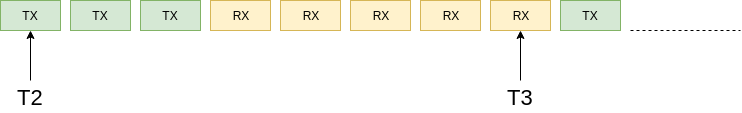
\includegraphics[width=\textwidth]{Figure/Sequence.png}
% \caption{Sequence of valid data packet with time}
% \label{sequence}
% \end{figure}
% \begin{figure}[h!]
% \centering
% 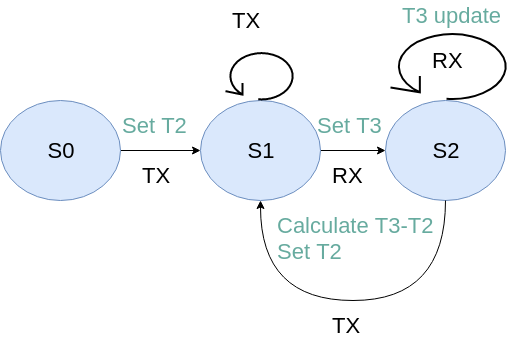
\includegraphics[scale=0.5]{Figure/State_Machine.png}
% \caption{State Machine}
% \label{state_machine}
% \end{figure}

% State Machine shown in Figure \ref{state_machine} controls the timing measurement function. It starts with state S0 and when it receives a TX event it sets T2 and moves to S1, further TX events don't update the value of T2 as we want the first TX event time. The state machine moves from S1 to S2 on a RX event, it sets the value of T3, further RX events updates the value of T3 as we want the time instant of the last RX event. On receiving TX event when at S2, it moves to S1, calculates $T3-T2$ and sets the value of T2.
% \subsection{Results Correlation Method}
% All the time instants are stored in Unix Time Format, a python script stores the values in separate arrays t1, t2, t3, t4 for GNU Radio Transmit Time, Kernel Transmit Time, Kernel Receive Time and GNU Radio Receive Time respectively. 



% Once the arrays have been compared to remove corrupt data, the mean and standard deviation of the respective arrays are found.
